\documentclass[a4paper,12pt, oneside]{article}
\usepackage[english]{babel}
\usepackage[utf8]{inputenc}
\usepackage[T1]{fontenc}
\usepackage{pdfpages}
\usepackage{csquotes}
\usepackage{dirtytalk}
\usepackage{graphicx}
\usepackage{wrapfig}
\usepackage{setspace}
\usepackage{listings}
\usepackage{mathtools}
\DeclarePairedDelimiter\ceil{\lceil}{\rceil}
\DeclarePairedDelimiter\floor{\lfloor}{\rfloor}
\graphicspath{ {figures/} }
\usepackage[colorlinks,allcolors=black]{hyperref}
\usepackage[algoruled,linesnumbered,noend]{algorithm2e}
\usepackage[parfill]{parskip}

\begin{document}

\begin{titlepage}
\begin{onehalfspace}
	\begin{wrapfigure}[4]{l}[22mm]{0.25\textwidth}
		\vspace*{-7mm}
		\centering
		
\includegraphics[width=0.25\textwidth]{bicocca.png}
	\end{wrapfigure}
	\par
	\noindent Università degli Studi di Milano Bicocca \\
	\textbf{Scuola di Scienze \\
			Dipartimento di Informatica, Sistemistica e Comunicazione \\
			Corso di laurea in Informatica}
\end{onehalfspace}

\vfill
\par

\begin{doublespace}
\begin{center}
	{\Huge \textbf{Algorithm Engineering: an algorithm for BWT and LCP}}
\end{center}
\end{doublespace}

\vfill
\par

\begin{onehalfspace}
\begin{flushleft}
	{\large \textbf{Relatore:} \textit{Prof. Gianluca Della Vedova} \\
			\textbf{Co-relatore:} \textit{Dott. Marco Previtali}}
\end{flushleft}

\vspace{8mm}
\par

\begin{flushright}
	{\large \textbf{Relazione della prova finale di:} \\
			\textit{Fabio Nicolini} \\
			\textit{Matricola 794467}}
\end{flushright}
\end{onehalfspace}

\vfill
\par

\begin{center}
	{\large \textbf{Anno Accademico 2016--2017}}
\end{center}

\end{titlepage}

\part*{Abstract}
\label{ch:Abstract}

\thispagestyle{empty}
This thesis describes problems, goals and achievements encountered while implementing an algorithm for computing the Burrows-Wheeler Transform (BWT) and Longest Common Prefix (LCP) exploiting external memory and minimizing the RAM usage.

The requirement of a low RAM usage for this task appears in fields where a large amount of data needs to be processed and manipulated, such as Computational Biology.

The introduction of more accessible DNA sequencing techniques made this constraint more impending: more data, composed of shorter but more numerous reads has highly increased the RAM usage of existent programs.

\newpage
\tableofcontents
\newpage

\section{Introduction}

The program discussed in this paper can be considered as a sub-routine of a larger project: a genome assembler implemented with the low RAM usage philosophy. BWT and LCP construction is a fundamental step towards developing of such software. Before discussing in detail the BWT and LCP construction we will introduce a very important aspect of computational biology: the origin of molecular sequence data, since string problems on such data provide a large part of the motivation for studying string algorithms in general.

\subsection{DNA sequencing}

The purpose of DNA sequencing is to determine the exact order of nucleotides within a DNA molecule. This task is of extreme importance and has application in many different fields: from molecular and evolutionary biology to medicine and forensics. It is in the essentially simple nature of the DNA that lies the fundamental structure of life:
\begin{displayquote}
The digital information that underlies biochemistry, cell biology, and development can be represented by a simple string of G's, A's, T's and C's. This string is the root data structure of an organism's biology. \cite{olsontimetosequence}
\end{displayquote}
The meeting point between biology and computer science is the assumption that biologically meaningful results could come from considering the DNA as a one-dimensional character string, abstracting away the reality of DNA as a flexible three-dimensional molecule.
To exactly determine this one-dimensional character string is not a simple task. Through exploiting an organism's biochemistry, it is possible to sequence its DNA in different ways, though all these techniques share similar problems; we will examine in detail a technique called \textit{shotgun sequencing}.
The main problem is that it's not possible to sequentially \say{read} many nucleotides, but at most a few hundred.(1000 - 1200 Sanger method, 50-500 NGS) \cite{gusfield} This is makes the sequencing task way more difficult and prompts to look for different approaches. Because of this issue it is not possible to reconstruct the DNA molecule starting from a single copy of such molecule. This is because even by fragmenting a single copy of DNA, there is not enough information to determine the order of the fragments. We will introduce a possible solution to this problem: the \textit{shotgun sequencing protocol}.

\subsubsection{Shotgun sequencing}

Shotgun sequencing is a protocol that has to be used in combination with other techniques that actually perform the reading task(like Sanger or NGS).
In fact, shotgun sequencing specifies \textit{how} to use the data read by other technologies in order to sequence large section of DNA.
The basic idea of this solution is to use multiple copies of the DNA of interest and then to cut these copies by physical, enzymatic, or chemical means so that each copy is cut in somewhat random locations. The cutting produces fragments from the original DNA, called \textit{reads}. In the fragmentation process the original order of the reads is lost, one simply is left with a set of reads without knowing their initial order in the full string nor from which copy of the string it came from. Still, the reads from different copies overlap each other so that if enough overlapping fragments are sequenced, the common patterns from overlapping sequenced fragments can be used to try assemble the sequence of the full DNA string (see figure).
\begin{figure}
	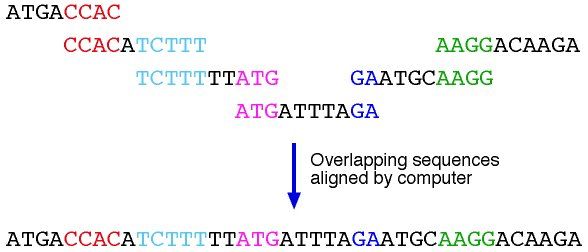
\includegraphics[width=0.7\textwidth]{seqoverlaps.jpeg}
	\centering
	\caption{Overlaps between fragments used to reconstruct original string}
	\label{fig:seqoverlaps}
\end{figure}
Hence the sequencing problem becomes something very similar to a \say{jigsaw puzzle} where the basic components are the DNA fragments randomly obtained from the DNA string, and the final picture to discover is the one-dimensional string representation of the DNA. This step is called \textit{sequence assembly}.

\subsection{Sequence assembly}

The problem of sequence assembly can be compared to taking many copies of a book, passing each of them through a shredder with a different cutter, and piecing the text of the book back together just by looking at the shredded pieces. Besides the obvious difficulty of this task, there are some extra practical issues: the original may have many repeated paragraphs, and some shreds may be modified during shredding to have typos. Excerpts from another book may also be added in, and some shreds may be completely unrecognizable. \cite{seqassemblywiki}
It is important to note that the sum of all nucleotides of all reads it's always much higher than the length of the reconstructed sequence. This means that there are always multiple different reads that contain the same nucleotide of the final sequence. Actually, very few of the fragments from the set of reads will be sequenced, since most procedures only sequence fragments of a fixed size range but the fragments' length is somewhat random. So instead of sequencing all the fragments, the shotgun technique randomly chooses fragments from the set of reads of an appropriate length and then it sequences the first $X$ bases, where $X$ is the fixed number used by the procedure (usually around 400 nucleotides). \cite{gusfield} 
\par
The number of fragments picked must be sufficient to allow reconstruction of the full DNA string from the overlapping sequenced parts of the fragments. Probabilistic analyses have been made \cite{mathangen} to determine how many fragments to pick. In practice, creation, cloning and selection of fragments is not always uniform enough to allow a complete reconstruction. This is one of the limits of the shotgun protocol, although the issue does not always lie in the probabilistic selection of reads but is due to molecular and biological reasons. In these cases even adding additional coverage does not solve the problem.
\par
Recalling the example of the book reconstruction, we said that there are some extra practical issues. These issues have a huge impact on the problem. For example, the reads may have wrong nucleobases (or missing ones) because the DNA sequencer does not always \say{read} them correctly. This makes the overlap detection a harder task since, if in reality two given reads should perfectly overlap, they may not because of some errors in the sequencing instrument. Another problem is the presence in the DNA molecule of identical or nearly identical sequences (known as \textit{repeats}). Given a read that is contained, even partially, inside one of these regions it's very difficult to determine the correct position of such read in the DNA string.
\par
Having briefly introduced DNA sequencing and sequence assembly, which comprise real front-line problems, we now step back a bit to introduce a more abstract pure string problem.

\subsubsection{Shortest superstring problem}

\begin{displayquote}
\textbf{Definition} \ \ \ Given a set of string $\Upsilon = \{S_1, S_2, ..., S_k\}$ a \textit{superstring} of the set $\Upsilon$ is a single string that contains every string in $\Upsilon$ as a substring.\\
\end{displayquote}

For example, a concatenation of the strings of $\Upsilon$ in any order gives a basic superstring of $\Upsilon$. For a more interesting example, let $\Upsilon = \{ \textit{actt, gtca, cttag} \}$. Then \textit{cttagacttgtca} is a superstring of $\Upsilon$, and \textit{gtcaacttag} is another, shorter superstring of $\Upsilon$. In general we are interested in finding superstrings whose length is small. This is because shorter superstrings take into consideration the overlaps between substrings and tend to unify them as one in the superstring. This is the way to go since, as explained before, overlapping sequences are likely to be in sequential ordering in the final superstring.
\par
The problem of finding the shortest superstring is mostly motivated by one approach to the sequence assembly problem in shotgun sequencing, although it may have other applications such as in data compression. The strings in the set $\Upsilon$ model the sequenced DNA fragments created by the shotgun sequencing protocol and the objective is to deduce the originating DNA string $S$ from the set of sequenced fragments $\Upsilon$.
Without sequencing errors, the full DNA string $S$ is a superstring of $\Upsilon$ and, under the assumptions stated above, $S$ is likely to be a shortest superstring of $\Upsilon$. Though most of the time $S$ will not be a very \say{good} string, as the model suggests. In fact, real sequence data indicates that the shortest superstring is often shorter than the originating string $S$, especially in presence of \textit{repeats}. Therefore the shortest superstring problem is an abstract algorithm that only loosely models the real sequence assembly task. Nonetheless it remains important to study abstract
approaches to practical problems because, more often than not, in the techniques and solutions to an abstract problem lies the key to obtain practical results in more complex or realistic systems. 
\par
The shortest superstring problem is known to be NP-hard \cite{computersintract}, therefore a polynomial-time algorithm to find the exact optimal is thought to be unlikely. Moreover, it has been found that the problem belongs to the MAX-SNP-hard complexity class \cite{linearssp}, and so it is also thought that there is no polynomial-time algorithm that can approximate the optimal time within an \textit{arbitrary, but predetermined} constant. However, several linear approximation have been proposed. The first by Blum et al. \cite{linearssp} guarantees an approximation factor of three. The factor has been successively improved many times; the best improvement to date, by Sweedyk\cite{scs25apprx} and Kaplan et al. separately\cite{scs25apprx2}, reduces the bound to 2.5. Nevertheless this is still an open problem because of the conjecture called \say{The Greedy Conjecture} that states: \textit{The Greedy Algorithm for the shortest superstring problem has an approximation factor of 2;} even though such an algorithm has not yet been discovered.
\par
A related problem that has interesting connection with the biological structure of the DNA molecule is the shortest superstring of a collection of strings where each string in the collection can be considered in both forward and backward orientation. This problem is motivated by the fact that most DNA molecules consist of two \textit{strands} coiled around each other to form a double helix, and the DNA fragments in real sequence assembly come from both strands, without exactly knowing the origin of any specific fragment.

\subsection{NGS introduction and its consequences}

Before next-generation sequencing was introduced the go-to technique was the Sanger method. It's the \say{original} sequencing technique that allowed for the first time to actually \textit{read} pieces of genetic material. However it soon became evident that the Sanger method was not ideal in order to sequence large sections of DNA. Even if the introduction of shotgun sequencing alongside the Sanger method solved the issue of sequencing larger section of DNA, it was still too slow and expensive. The revolution was the introduction of NGS (Next Generation Sequencing) technologies. The core philosophy of massive parallel sequencing use in NGS is adapted from shotgun sequencing. The read length (actual number of continuous sequenced bases) for NGS is much shorter than that attained by Sanger sequencing.\cite{impactofngs} In this aspect Sanger sequencing performs better than NGS but the other advantages achieved by using NGS make up for this disparity. NGS technologies have demonstrated the capacity to sequence DNA at unprecedented speed, thereby enabling previously unimaginable scientific achievements. But the massive data produced by NGS also presents a significant challenge for data storage, analyses, and management solutions. Advanced bioinformatics tools are essential for the successful application of NGS technology. \cite{impactofngs}

\newpage
\section{Data structures in Bioinformatics}

A relevant aspect of Bioinformatics is the large quantity of data it needs to manage. This prompted since the beginning of the \say{Bioinformatics era} the need to find efficient ways to manipulate huge datasets. From a programming point of view this is translated in finding efficient data structures that properly represent the biological data. Finding efficient data structures not only reduces the storage/memory usage, which is the primary objective of the algorithm implemented in this paper, but it usually even enhances time performance. For example when a program does a large amount of Input/Output operations, compressing the data enhances both space and time efficiency. In this sense, data structures for compression and indexing are important area of research. Before analyzing the more complex data structures constructed by our algorithm we will introduce two data structures of fundamental importance in computational biology, on which the LCP-array and the BWT are based.

\subsection{Suffix tree}

A suffix tree is a data structures that exposes the internal structure of a string. Strings are the base components that basically every computational biology algorithm needs to manipulate. In particular the classic application for suffix trees is the \textit{substring problem}.\cite{gusfield} The substring problem consists in finding out if a given string $S$ is contained (i.e. it's a substring), in a longer string $T$ called \textit{text}. Let $m$ and $n$ be the length of $T$ and $S$ respectively. After $\mathcal{O}(m)$, or linear, preprocessing time, one must be able to take in any random string $S$ and in $\mathcal{O}(n)$ time either find an occurrence of $S$ in $T$ or determine that $S$ is not contained in $T$. This means that the preprocessing time takes time proportional to the length of the text, but after that, the search of $S$ is done in time proportional to the length of $S$, \textit{independent} of the length of $T$. These bounds are achieved with the use of a suffix tree. The suffix tree is built in $\mathcal{O}(m)$ time, and exposes important information about the text string in the preprocessing phase. Thereafter, whenever a string of length $\mathcal{O}(n)$ is input, the algorithm searches for it in $\mathcal{O}(n)$ time using that suffix tree. 
\par
The concept of suffix tree was first introduced by Weiner \cite{suffixtreeweiner} in 1973. The construction was, since then, simplified many times. First by McCreight \cite{suffixtreemccreight} and then by Ukkonen \cite{suffixtreeukkonen}. All these algorithms have a linear running time for fixed alphabets, and a general worst-case running time of $\mathcal{O}(n \log n)$. Farach \cite{suffixtreefarach} gave the first suffix tree construction that is optimal for all alphabets. In particular, his solution was the first one to be optimal for alphabets over integers in a polynomial range. We will not examine these more complex linear-time suffix tree construction algorithms, but we will show a naive method that has a quadratic running time.

\subsubsection{Basic definitions}
Suffix trees are used in a wide range of application, therefore we will not refer to the starting string as $T$ (text) but as the more general and abstract string $S$. The alphabet is assumed finite and known.
\begin{itemize}
	\item The \emph{suffix} and \emph{prefix} of length $l$ of a generic $m$-character string $S$ are the substrings $S[m-l +1: m]$ (denoted by $S[m-l +1:]$) and $S[1: l]$ (denoted by $S[:l]$) respectively. Then the \emph{$l$-suffix} and \emph{$l$-prefix} of a string $S$ is the suffix and prefix with length $l$, respectively \cite{paper}.
	\item A suffix tree $Z$ for $S$ is a rooted directed tree with exactly $m$ leaves numbered from 1 to $m$.
	\item Each internal node, other than the root, has at least 2 children and each edge is labeled with nonempty substring of $S$.
	\item No two edges out of a node can have edge-labels beginning with the same character.
	\item The string obtained by concatenating all the string-labels found on the path from the root to leaf $i$ spells out the suffix of $S$ that starts at position $i$. That is, it spells out $S[i...m]$.
\end{itemize}

This definition of a suffix tree does not guarantee the existence of a suffix tree for any string $S$. Problems arise when one \textit{suffix} of $S$ matches a \textit{prefix} of another suffix of $S$. In this case the path of the first suffix would not end at a leaf. This definition guarantees the existence of a suffix tree only for those strings in which the last character does not appear in the rest of the string. So, a solution to the problem is extending the string $S$ with an additional character at the end, called termination symbol, that is not in the same alphabet that $S$ is taken from. The usage of a termination symbol is common practice in computational biology problems and, as usual in bioinformatics literature, we will use the symbol '\$' . From now on every string $S$ is assumed to be extended with the termination symbol \$, even if not explicitly shown.\\

\newpage
\textbf{Definitions}
\begin{itemize}
	\item Consider a path from the root that ends at a node. The \textit{label of a path} of that path is the ordered concatenation of the substrings labeling the edges of that path.
	\item Given a node $v$, the \textit{string-depth} of $v$ is the length of $v$'s label.
\end{itemize}

We will know show how the exact matching problem on a text $T$ can be easily solved when possessing the correspondent suffix tree $Z$.

\subsubsection{Suffix trees and exact matching}
Given a pattern $P$ of length $n$ and a text $T$ of length $m$ suffix trees can be used to find all occurrences of $P$ in $T$ in $\mathcal{O}(n + m)$ time:


\begin{displayquote}
Build a suffix tree $Z$ for text $T$ in $\mathcal{O}(m)$ time. Then, match the characters of $P$ along the unique path in $Z$ until either $P$ is exhausted or no more matches are possible. In the latter case, $P$ does not appear anywhere in $T$. In the former case, every leaf in the subtree below the point of the last match is numbered with a starting location of $P$ in $T$, and every starting location of $P$ in $T$ numbers such a leaf. \cite{gusfield}
\end{displayquote}

\begin{figure}
	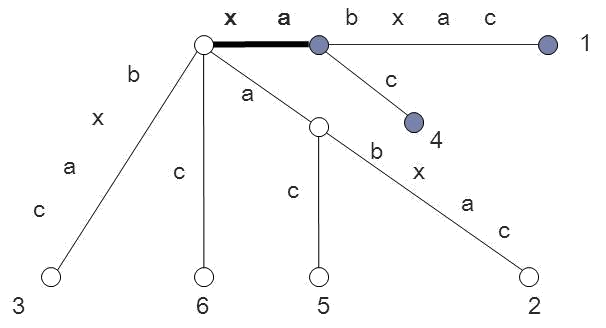
\includegraphics[width=0.8\textwidth]{suffix-trees-pattern-matching.png}
	\centering
	\caption{T = $xabxac$, P = $xa$. We can deduce that the pattern occurs in the text starting at positions 1 and 4}
	\label{fig:suffixtreematching}
\end{figure}

The latter case is pretty simple. By traversing the suffix tree down from the root along the path which label matches the pattern, if at some point $P$ is not exhausted but still there are no matching paths out of the current node, it clearly means that $P$ is nowhere to be found in $T$ since it \textit{doesn't match any prefix of any suffix}. The key to understanding the former case (when at some point $P$ is exhausted) is to note that $P$ occurs in $T$ starting at position $j$ if and only if $P$ occurs as a prefix of the suffix $T[j..m]$. This happens if only if $P$ labels at least an initial part of a path from the root to leaf $j$. If $P$ is exhausted then $P$ occurs somewhere in $T$.
If $P$ is exhausted at the \say{end} of the tree, i.e. at a leaf, then $P$ occurs in $T$ only once starting at the position that corresponds to the numeration of the leaf. Otherwise, if $P$ is exhausted at a non-leaf node (see Figure 2) $P$ occurs multiple times in $T$; precisely $P$ occurs in $T$ a number of times equal to the number leafs in the subtree rooted at the node where $P$ is exhausted. If this is the case, the algorithm can find all the starting positions of $P$ in $T$ by traversing the subtree below the end of the matching path, collecting position numbers written at the leaves. All occurrences of $P$ can therefore be found in $\mathcal{O}(n+m)$ time. 
\par
There are further improvements to this method that will not be discussed; instead we will conclude the discussion on suffix trees by showing a simple algorithm for suffix tree construction in quadratic time.

\subsubsection{Simple suffix tree construction algorithm}
Given a string $S$ of length $m$ this simple method first enters a single edge for suffix $S[1..m]\$$ (the entire string) into the tree. Afterwards it iteratively enters suffix $S[i..m]\$$ into the tree, for $i$ increasing from 2 to $m$. Let $N_i$ denote the intermediate tree that encodes all the suffixes from 1 to $i$. In detail $N_1$ consists of a single edge between the root and a leaf labeled 1. The edge is labeled with the string $S\$$. Tree $N_i+1$ is constructed from $N_i$ as follows: 

\begin{displayquote}
Starting at the root of $N_i$ find the longest path from the root whose label matches a prefix of $S[i+1..m]\$$. This path is found by successively comparing and matching characters in suffix $S[i+1..m]\$$ to characters along a unique path from the root, until no further matches are possible. The matching path is unique because no two edges out of a node can have labels that begin with the same character. At some point, no further matches are possible because no suffix of S\$ is a prefix of any other suffix of S\$. When that point is reached, the algorithm is either at a node, $w$ say, or it is in the middle of an edge. If it is in the middle of an edge, $(u, v)$ say, then it breaks edge $(u, v)$ into two edges by inserting a new node, called $w$, just after the last character on the edge that matched a character in the current suffix($S[i+1..m]\$$). The new edge $(u, w)$ is labeled with the part of the $(u, v)$ label that matched with $S[i+1..m]\$$, and the new edge $(w, v)$ is labeled with the remaining part of the $(u, v)$ label. Then (whether a new node $w$ was created or whether one already existed at the point where the match ended), the algorithm creates a new edge $(w, i+1)$ running from $w$ to a new leaf labeled $i+1$, and it labels the new edge with the unmatched part of suffix $S[i+1..m]\$$. \cite{gusfield}.
\end{displayquote}
The tree now contains a unique path from the root to leaf $i+1$, and this path has the label $S[i+1..m]\$$. Assuming a bounded-size alphabet, the above naive method take $\mathcal{O}(m^2)$ time to build a suffix tree for the string $S$ of length $m$.
\par
We will now introduce suffix arrays, a more space efficient data structure based on suffix trees that has important relations with the LCP-array constructed by the algorithm described in this paper.

\subsection{Suffix array and LCP}
One of the most important properties that suffix arrays have but suffix trees don't is the \textbf{alphabet independence}. Time and space bounds for most strings problems are influenced by the size of the alphabet $\Sigma$, the larger the alphabet, the larger the problem. For that reason, sometimes it is explicitly referred to those time and space bounds in terms of alphabet size ($|\Sigma|$). In this case, we would refer to the construction time for suffix tree as $\mathcal{O}(m\log|\Sigma|)$, where $m$ is the size of the string. More completely the Weiner, Ukkonen, and McCreight algorithms that we briefly mentioned all either require $\Theta(m|\Sigma|)$ space, or the $\mathcal{O}(m)$ time bound should be replaced with the minimum of $\mathcal{O}(m\log m)$ and $\mathcal{O}(m \log |\Sigma|)$. Similarly, searching for a pattern $P$ using a suffix tree can be done with $\mathcal{O}(|P|)$ comparisons only if we use $\Theta(m|\Sigma|)$ space, otherwise we must allow the minimum of $\mathcal{O}(|P|\log m)$ and $\mathcal{O}(|P|\log |\Sigma|)$ comparisons during each search. For these reasons, a suffix tree may require too much space to be practical in some applications.
In the context of the substring problem, a fixed string $T$ will be searched many times. In this case the most important bounds are:
\begin{itemize}
	\item Time needed for the search of the pattern in the text.
	\item Space used by the fixed data structure representing $T$.
\end{itemize}

The space used in the construction of the data structure representing $T$ is not critical, although it should be still \say{reasonable}.
Usually these two bounds are not completely unrelated, in fact a very space efficient data structure is often the cause of a time-complexity improvement.
In 1993 Manber and Myers \cite{suffixarray} proposed a new data structure, called \textit{suffix array}, that is very space efficient, yet contains useful information about the internal structure of a string. These informations can be used to efficiently solve many string problems, in particular the exact matching problem, almost as efficiently as with a suffix tree. \newline \newline
\textbf{Definition} 
\begin{itemize}
	\item Given a $m$-character string $T$, a \textbf{suffix array} for $T$, called $A$, is an array of the integers in the range 1 to $m$, specifying the lexicographic order of the $m$ suffixes of string $T$.
\end{itemize}

That is, the suffix starting at position $A(1)$ of $T$ is the lexically smallest suffix. In general suffix at position $A(i)$ is lexically less than suffix at position $A(i+1)$. Even in this contest every string should be assumed extended with the termination symbol $\$$, which is considered to be lexically \textit{less} than any other character in the alphabet. \newline
Example of a suffix array for $T = banana$:

\begin{table}[h!]
\centering
\label{suffix-array1}
\begin{tabular}{llllllll}
$i$ & 1 & 2 & 3 & 4 & 5 & 6 & 7 \\
\hline
$T[i]$ & b & a & n & a & n & a & \$
\end{tabular}
\end{table}

The text has the following suffixes:

\begin{table}[h!]
\centering
\label{suffix-array2}
\begin{tabular}{ll}
$Suffix$   & $i$ \\
\hline
banana\$ & 1 \\
anana\$  & 2 \\
nana\$   & 3 \\
ana\$    & 4 \\
na\$     & 5 \\
a\$      & 6 \\
\$       & 7
\end{tabular}
\end{table}

\newpage
The suffixes can be sorted in ascending order:

\begin{table}[h!]
\centering
\label{suffix-array3}
\begin{tabular}{ll}
$Suffix$   & $i$ \\
\hline
\$       & 7 \\
a\$      & 6 \\
ana\$    & 4 \\
anana\$  & 2 \\
banana\$ & 1 \\
na\$     & 5 \\
nana\$   & 3
\end{tabular}
\end{table}

The \textbf{suffix array} $A$ contains the starting positions of these sorted suffixes:

\begin{table}[h!]
\centering
\label{suffix-array4}
\begin{tabular}{llllllll}
$i$ & 1 & 2 & 3 & 4 & 5 & 6 & 7 \\
\hline
$A[i]$ & 7 & 6 & 4 & 2 & 1 & 5 & 3
\end{tabular}
\end{table}

Notice that the suffix array holds only integers and hence contains no information about the alphabet used in string $T$. Therefore the space required by suffix arrays is modest: for a string of length $m$, the array can be stored in exactly $m$ computer words, assuming a word of at least $\log m$ bits. \par
In combination with the LCP-array, that consists of another $2m$ values, the suffix array can be used to find all occurrences in $T$ of a pattern $P$ in $\mathcal{O}(n+\log_2 m)$ single-character comparison and bookkeeping operations. Moreover, this bound is independent of the alphabet size. Since for most problems of interest $\log_2 m$ is $\mathcal{O}(n)$, the substring problem is solved by using suffix arrays as efficiently as by using suffix trees \cite{gusfield}.

Suffix arrays are closely related to suffix trees:

\begin{itemize}
	\item Suffix arrays can be constructed by performing a depth-first (i.e. linear time) traversal of a suffix tree. The suffix array corresponds to the leaf-labels given in the order in which these are visited during the traversal, if edges are visited in the lexicographical order of their first character.
	Nevertheless it's possible, and more efficient, to build a suffix array without first constructing a suffix tree and then converting it to a suffix array.
	\item It has been shown \cite{abouelhoda} that suffix arrays enhanced with additional information (like the LCP-array) can solve the same problems as suffix trees in the same time complexity.
\end{itemize}

\newpage
\textbf{Definition}

\begin{displayquote}
$Lcp[i, j]$ is the length of the longest common prefix of the suffixes specified in positions $i$ and $j$ of $A$. That is, $Lcp[i, j]$ is the length of the longest prefix common to suffix $A[i]$ and suffix $A[j]$.
\end{displayquote}

The \textbf{LCP-array} was first introduced as a \say{super accelerant} for exact string matching as support to the suffix-array. In this case the LCP-array values are computed in the preprocessing phase. In fact it is possible to compute the LCP during the depth-first tree traversal used to build the suffix array. LCP values are used in the exact matching algorithm to skip as many character comparison as possible; since $Lcp[i, j]$ indicates the number of consecutive initial character common to two strings (suffix $A[i]$ and suffix $A[j]$), it directly indicates how many comparison can be skipped. \par
The LCP has other important application in computational biology and not always as support to the suffix array. In fact, in certain applications, the space requirements of suffix arrays may \textit{still be prohibitive}. Such requirements motivated the development of even more space-efficient data structures, some of which are based on the BWT, like the FM-index. Some fundamental bioinformatics problems such as genome assembly, require an all-against-all comparison among the input strings, especially to find all prefix-suffix matches (or overlaps) between reads in the context of the Overlap-Layout-Consensus (OLC) approach based on string graph \cite{stringgraphs}. This fact justifies to search for extremely efficient algorithms to compute the BWT and the LCP array on a collection of strings.

\subsection{BWT}
The \textbf{Burrows-Wheeler Transform} is a \textit{reversible} transformation of a string. It was first introduced in 1994 \cite{bwt} and its first application was in data compression. The BWT by itself does \textbf{not} perform the compression, it simply \textit{permutes} the order of the character of the string. The permutation is done in order to facilitate the string's compression. This happens because the BWT exposes repeated similarities inside the string. For example, if the original string had several substrings that occurred often, then the transformed string will have several places where a single character is repeated multiple times in a row. This is useful for compression, since techniques like move-to-front transform and run-length encoding, can easily exploit repeated sequences of characters inside a string \cite{bwt}. Furthermore the transformation is \textbf{reversible}, without needing to store any additional data. This makes the BWT a space-free improvement to compression algorithms, and the additional computation required for the BWT construction is a convenient trade-off.
One of the most important compression programs that uses the BWT as its core subroutine is bzip2 \cite{bzip2}. \newline

The actual transformation is done as follows:

\begin{itemize}
	\item Generation of all possible rotations of the text and creation of a matrix in which every rotation is a row.
	\item Sorting the rows (i.e. rotations) by lexicographic order.
	\item The BWT is the last column of the resulting matrix.
\end{itemize} 

Example for $T = BANANA\$$, where \$, as usual, indicates end of the string. In this example as well, we follow the convention that the symbol \$ is lexically less of any character of the alphabet.

\begin{table}[h!]
\centering
\label{bwt-example}
\begin{tabular}{lllll}
Input    & All rotations                                                                                                & Lexical sorting                                                                                              & Last column                                                                                                  & Output   \\ \hline
BANANA\$ & \begin{tabular}[c]{@{}l@{}}BANANA\$\\ \$BANANA\\ A\$BANAN\\ NA\$BANA\\ ANA\$BAN\\ NANA\$BA\\ ANANA\$B\end{tabular} & \begin{tabular}[c]{@{}l@{}}\$BANANA\\ A\$BANAN\\ ANA\$BAN\\ ANANA\$B\\ BANANA\$\\ NA\$BANA\\ NANA\$BA\end{tabular} & \begin{tabular}[c]{@{}l@{}}\$BANAN\textbf{A}\\ A\$BANA\textbf{N}\\ ANA\$BA\textbf{N}\\ ANANA\$\textbf{B}\\ BANANA\textbf{\$}\\ NA\$BAN\textbf{A}\\ NANA\$B\textbf{A}\end{tabular} & \textbf{ANNB\$AA}
\end{tabular}
\end{table}

The BWT of a string $T$ is strictly related to the suffix array of $T$. In fact, the $i$-$th$ symbol of the BWT is the symbol preceding the $i$-$th$ smallest suffix of $T$ according to the lexicographic sorting of the suffixes of $T$.\par 
The Burrows-Wheeler Transform has gained importance beyond its initial purpose, and has become the basis for self-indexing structures such as the FM-index \cite{ferraginafmindex}.
It is important to note that the algorithm described constructs the BWT of a \textit{collection} of strings, which is a generalization of the procedure described above. One of the advantage of the new theoretical approach discussed in \cite{paper} is that it facilitates the extension to a collection of variable-length strings . This possible further improvement is briefly discussed in the final section of this paper, but it is important to note that the implementation is based on the less general case of same-length string collection.



\newpage
\section{Algorithm description}
Here we report the algorithm formalization as introduced in \cite{paper}. The algorithm computes the Burrows-Wheeler Transform and the Longest Common Prefix array for a collection of string in external memory. Among the first efficient algorithms for this task there are BCRext\cite{bcrext} and extLCP\cite{extlcp} for BWT and LCP construction respectively. The method described here aims to be an efficient alternative to those approaches.

\subsection{Basic concepts}

Let $\Sigma = \{c_0, c_1,...,c_\sigma\}$ be a finite alphabet where $c_0 = \$$ (termination symbol), and $c_0 < c_1 < ... < c_\sigma$ where $<$ specifies the lexicographic ordering over alphabet $\Sigma$. We consider a collection $S = \{s_1, s_2,...,s_m\}$ of $m$ strings, where each string $s_j$ consists of $k$ symbols over the alphabet $\Sigma\setminus\{\$\}$ and is terminated by the symbol $\$$. As already discussed, $k$ is assumed fixed for every string in the collection.


\subsubsection{Auxiliary definitions}

\begin{itemize}
	\item $s_j[i]$ denotes the $i$-$th$ symbol of string $s_j$.
	\item $s_j[i:t]$ denotes the substring containing the consecutive characters from position $i$ to $t$ of $S_j$.
	\item Let $V$ be a generic vector, we denote with $V[1:q]$ the first $q$ elements of $V$ and with $rank_V(q, x)$ the number of elements equals to $x$ in $V[1:q]$.
	\item Let $X$ be the lexicographic ordering of the suffixes of the collection $S$. The \textit{Suffix Array} $A$ is the $m(k+1)$-long array where $A[i] = (p, j)$ if and only if the $i$-th element of $X$ is the $p$-suffix of string $s_j$.
	\item The \textit{Burrows-Wheeler Transform} of $S$ is the $m(k+1)$-long array $B$ where if $A[i] = (p, j)$ then $B[i]$ is the first symbol of the $(p+1)$-suffix of $s_j$ if $p < k$, otherwise $B[i] = \$$. In other terms $B$ consists of the symbols preceding the ordered suffixes of $X$, where the symbol $\$$ is also the one that precedes each string $s_i\in S$.
	\item The \textit{Longest Common Prefix array} of $S$ is the $m(k+1)$-long array $LCP$ such that $LCP[i]$ = 	length of the longest prefix shared by suffixes $X[i-1]$ and $X[i]$. Conventionally, $LCP[1] = -1$.

\end{itemize}	


\subsection{BWT construction: Interleave}

The construction of the BWT extensively uses the notion of \textit{interleave}. In particular the algorithm computes the BWT starting from two elements: The \textbf{partial}-BWT and the encoding $I_W$. The partial-BWT is a collection of $k+1$ arrays of characters and the \textit{interleave-encoding} $I_W$ is an array of $m(k+1)$ integers. In simple terms, the \textbf{interleave} of the $k+1$ arrays is the result of merging those arrays \say{mediated} by the interleave encoding. In this algorithm the BWT corresponds to the interleave of the partial-BWT and the encoding $I_W$.
%skipped formal definition
\par
More formally, the interleave $W$ of a generic set of arrays $V_0,V_1,...,V_n$ is an array giving a fusion of $V_0, V_1, \ldots, V_n$ which preserves the relative order of the elements in each one of the arrays. As a consequence, for each $i$ with $0 \leq i \leq n$, the $j$-${th}$ element of $V_i$ corresponds to the j-${th}$ occurrence in $W$ of an element of $V_i$. This fact allows the $I_W$ array the encode the information that $I_W[q] = i$ if and only if $W[q]$ is an element of $V_i$. By observing that $W[q]$ is equal to $V_{I_W[q]}[j]$ where $j = rank_{I_W}(q, I_{W}[q])$, it is easy to show how to reconstruct $W$ from $I_W$ (see Algorithm~\ref{alg:interleave-encoding} where the array $pos[i]$ at line \ref{alg:interleave-encoding:element} is equal to $rank_{I_W}(q, i)$).

Figure~\ref{fig:interleave} shows an example of an interleave of four arrays $V_0, V_1, V_2, V_3$ and its encoding.

\begin{figure}[htbp]
  \centering
    \begin{minipage}{0.3\textwidth}%
  \begin{tabular}{|c|c|c|c|}
\hline
$V_{0}$&$V_{1}$&$V_{2}$&$V_{3}$\\\hline
T&C&A&A\\
T&G&C&A\\
A&G&C&T\\
\hline
\end{tabular}
  \end{minipage}%
  \quad%
    \begin{minipage}{0.3\textwidth}%
  \begin{tabular}{|c|c|}
    \hline
    $W$&$I_{W}$\\\hline
    T&0\\
    A&2\\
    A&3\\
    A&3\\
    C&1\\
    C&2\\
    C&2\\
    G&1\\
    G&1\\
    T&0\\
    A&0\\
    T&3\\
\hline
\end{tabular}
\end{minipage}
\caption{Example of an interleave $W$ of four arrays $V_0, V_1, V_2, V_3$.}
	\label{fig:interleave} 
\end{figure}
 
\begin{algorithm}[htb!]
	\For{$i\gets 0$ to $n$}{%
		$pos[i] \gets 0$\;
	}

	\For{$q \gets 1$ to $|I_W|$}{%
		$i \gets I_W[q]$\;
		$pos[i] \gets pos[i] +1$\;
		$W[q] \gets V_i[pos[i]]$\;\label{alg:interleave-encoding:element}
	}
	
	\caption{Reconstruct the interleave $W$ from the encoding $I_W$}
	\label{alg:interleave-encoding}
\end{algorithm}
\newpage

\subsection{Sketch of the algorithm}

Let $X_l$ and $B_l$, with $0 \leq l \leq k$, be the arrays of length $m$ such that $X_l[i]$ is the $i$-$th$ smallest $l$-suffix of $S$ and $B_l[i]$ is the symbol preceding $X_l[i]$. In particular $X_0$ and $B_0$ respectively list the $0$-suffixes and the last characters of the input strings in their order in the set $S$. It follows that $B_l$ is a subsequence of the BWT $B$ of $S$. Furthermore $B$ is an interleave of the $k+1$ arrays $B_0, B_1,...,B_k$. Similarly, the lexicographic ordering $X$ of all suffixes of $S$ is an interleave of the arrays $X_0, X_1, ..., X_k$. Let $I_B$ be the encoding of the interleave of arrays $B_0, B_1,...,B_k$, giving the BWT B, and let $I_X$ be the encoding of the interleave of arrays $X_0, X_1, ..., X_k$, giving $X$. Then it's possible to show that $I_B = I_X$ \cite{paper}. The algorithm exploits this property to compute the BWT as an interleave of $I_X$, instead of using $I_B$. Moreover $I_X$ can be simultaneously used to compute the LCP array as well. \par
The algorithm, differently from BCRext and extLCP, consists of two different phases: in the first phase the partial BWTs $B_0, B_1,...,B_k$ are computed (see section Section~\ref{partbwtcompute}), while the second phase (Section~\ref{secondphase}) is based on the Holt-McMillan approach \cite{interleave} and determines $I_X$, thus allowing to reconstruct $B$ as an interleave of $B_0, B_1,...,B_k$. In particular the method consists in an external memory radix-sort approach realized by using lists, which can be implemented in files. In order for the implementation to be efficient in contexts were  Hard Drives are used (in contrast to Solid-State Drives) every file (list) is accessed sequentially.


\newpage
\subsection{Partial BWT computation}
\label{partbwtcompute}

First the input strings $s_1, ..., s_m$ are preprocessed in order to compute $k+1$ arrays $T_0, T_1, ..., T_k$ with length $m$.

\begin{itemize}
	\item $T_l$ lists the characters in position $k-l$ of the input strings, such that $T_l[i] = s_i[k-l]$ when $0 \leq l \leq k-1$ and $T_l[i] = \$$ when $l = k$.
\end{itemize}

It follows that $T_l[i]$ is the symbol preceding the $l$-suffix of $s_i$. Clearly, those arrays can be computed in $\mathcal{O}(km)$ time and $\mathcal{O}(km\log \sigma)$ I/O complexity by sequentially reading the input strings.
Then Algorithm~\ref{alg:sort-suffixes} computes the partial BWTs $B_0, B_1,...,B_k$ by receiving in input the arrays $T_0, T_1,...,T_k-1$ and by using $k+1$ arrays $N_l$ with length $m$ ($0 \leq l \leq k$), defined as follows:

\begin{itemize}
	\item $N_l[i] = q$ if and only if the $i$-$th$ element of $X_l$ is the $l$-suffix of the input strings $s_q$.
\end{itemize} 

Note that $B_l[i] = s_q[k-l]$ and when $l = k$, $B_k[i] = \$$. In particular, $N_0$ is the sequence of indexes $\langle 1,2,3,...,|S|\rangle$ and $B_0$ is the sequence $\langle s_1[k], s_2[k],...,s_m[k]\rangle$ of the last symbols of the input strings (i.e. the symbols before the sentinels); that is $B_0 = T_0$. 
So, the algorithm starts with $B_0$ and $N_0$. At each iteration $l$, $B_l$ is computed from $N_l$ which in turn is computed with the support of the set of lists, $\cal P$ $(c_h)$ = \{$\cal P$$(c_0)$, $\cal P$$(c_1)$, ..., $\cal P$$(c_\sigma)$\} where $c_0, c_1, ..., c_\sigma$ is the lexicographic order of symbols in $\Sigma$ (i.e. $0 \leq h \leq |\Sigma|$). $N_l$ will be the result of the \textit{ordered concatenation} of each lists in $\cal P$ $(c_h)$ . This set is created as follows:

\begin{itemize}
	\item We perform a linear scan of $B_{l-1}$. Let $i$ be the index of this scan and let $c_h = B_{l-1}[i]$.
	\item We append the integer $N_{l-1}[i]$ to $\cal P$ $(c_h)$, where $c_h = B_{l-1}[i]$.
	\item $N_l$ is then obtained as the concatenation of $\cal P$$(c_0)$, $\cal P$$(c_1)$, ..., $\cal P$$(c_\sigma)$.
	\item Finally we compute $B_l$ by performing another linear scan but this time of the freshly calculated $N_l$. Let $q = N_l[i]$, then $B_l[i] = T_l[q]$.
\end{itemize}


Observe that also the array $B_l$ and $N_l$ of each iteration can be stored in lists (implemented in files) since they are sequentially accessed. Due to random access, for each $l$ (loop at line 4) the array $T_l$ is kept in RAM, but in different iterations of the loop, with a total space cost of $O(m \log \sigma)$. 

Algorithm~\ref{alg:sort-suffixes} describes this procedure in detail.

\newpage
\begin{algorithm}[htb!]
	\SetKwInOut{Input}{Input}\SetKwInOut{Output}{Output}
	\Input{The arrays $T_0, \ldots, T_{k}$}
	%\Output{The arrays $B_0, \ldots, B_k$}
	%$\mathcal{B}_0 \gets$ empty list\;
	%$\mathcal{N}_0 \gets$ empty list\;
	\For{$i\gets 1$ to $m$}{%
		$B_0[i] \gets T_0[i]$\;
		$N_0[i] \gets i$\;
	}
	\For{$l\gets 1$ to $k$}{%
		\For{$h\gets 0$ to $\sigma$}{%
			${\cal P}(c_h) \gets $ empty list\;
		}
		\For{$i\gets 1$ to $m$}{\label{alg:sort-suffixes:compute-projections-start}%
			$c_h \gets B_{l-1}[i]$\;
			$q \gets N_{l-1}[i]$\;
			Append $q$ to  ${\cal P}(c_h)$\; \label{alg:sort-suffixes:compute-projections-end}
		}
		$N_l \gets {\cal P}(c_0){\cal P}(c_1)\cdots{\cal P}(c_{\sigma})$\;\label{alg:sort-suffixes:compute-N}
		\For{$i\gets 1$ to $m$}{\label{alg:sort-suffixes:compute-B-start}%
			$q \gets N_l[i]$\;
			$B_l[i] \gets T_{l}[q]$\;\label{alg:sort-suffixes:compute-B-end}
		}
	}
	%\caption{Partition-suffixes}
	\caption{Compute the partial BWTs $B_0, B_1, \cdots, B_k$}
	\label{alg:sort-suffixes}
\end{algorithm}



\subsection{From the partial BWT to the $I_X$ encoding and the LCP array
\label{secondphase}}

In this section we will describe the second step of the algorithm that computes the BWT $B$ and the LCP array. In order to compute the BWT $B$ the only element needed at this point of the algorithm is the encoding $I_X$, since phase 1 already computed the partial BWTs $B_0, B_1,...,B_k$. In this paper we will not provide a formal proof of correctness for the algorithm; this can be found in \cite{paper}. The main idea in this phase is inspired from radix sort, that is to iteratively perform scans on the set of suffixes such that the overall ordering of the suffixes converges to their lexicographic order. Similarly to phase one, the $I_X$ encoding and the LCP array will be computed iteratively.
Each iteration $p$ computes $I_{X_{p+1}}$ and $LCP_{p+1}$ from $I_{X_p}$ and $LCP_p$ respectively. Similarly to the partial BWT computation, even $I_{X_{p+1}}$ and $LCP_{p+1}$ are constructed as the ordered concatenation of $\sigma + 1$ additional lists generated at every iteration from the partial BWT and $I_{X_p}$ or $LCP_p$ for BWT and LCP respectively. They key problem now becomes how are these $\sigma + 1$ lists created; we will separately show their construction.

\begin{algorithm}[tb!]
  \SetKwInOut{Input}{Input}\SetKwInOut{Output}{Output}
 
	$\mathcal{I}(c_0) \gets 0,0, \cdots, 0$\;
	$\mathcal{I}(c_1), \ldots, \mathcal{I}(c_{\sigma}) \gets $ empty lists\;
	$\mathcal{L}(c_0) \gets -1,0, \cdots, 0$\;
	$\mathcal{L}(c_1), \ldots, \mathcal{L}(c_{\sigma}) \gets $ empty lists\;

  %$L(\$) \gets $ the list $<-1>$\label{alg:compute-by-offset-with-lcp:init1}\;
  \ForEach{$c\in \{c_1, \cdots, c_{\sigma}\}$}{%
    $\mathcal{L}(c) \gets $ the list $<0>$\label{alg:compute-by-offset-with-lcp:init2}\;
  }
  
  $\alpha \gets \{-1,-1, \ldots, -1\}$\;\label{alg:compute-by-offset-with-lcp-init-alpha}
  
  \For{$i\gets 1$ to $|I_{X^{p}}|$}{%
    $l \gets I_{X^{p}}[i]$\;
    $c \gets B_l[rank_{I_{X^p}}(i,l)]$\tcp*{is the character preceding the
      current suffix}
	\If{$c \ne \$$}{
    	Append $(l+1)$ to $\mathcal{I}(c)$\;\label{alg:compute-by-offset-with-lcp:append}
    	}
    
    $lcp \gets LCP_{p}[i]$\;

    \ForEach{$d\in \{c_1 \cdots, c_{\sigma}\}$}{\label{alg:compute-by-offset-with-lcp-update-alpha}
      $\alpha[d] \gets \min\{\alpha[d], lcp\}$\;\label{alg:compute-by-offset-with-lcp-update-alpha-end}
    }
    
    \If{$c \ne \$$ and $\alpha[c] \ge 0$\label{alg:compute-by-offset-with-lcp:compute-lcp}}{%
      Append $\alpha[c] + 1$ to $\mathcal{L}(c)$\;
    }

    $\alpha[c] = \infty$\;
    
  }
  $I_{X^{p+1}} \gets \mathcal{I}(c_0) \mathcal{I}(c_1) \cdots \mathcal{I}(c_{\sigma})$\;
  $LCP_{p+1} \gets \mathcal{L}(c_0) \mathcal{L}(c_1) \cdots \mathcal{L}(c_{\sigma})$\;\label{alg:compute-by-offset-with-lcp-concat}

\caption{Compute $I_{X^{p+1}}$ and $LCP_{p+1}$ from $I_{X^{p}}$ and $LCP_{p}$}
\label{alg:compute-by-offset-with-lcp}
\end{algorithm}

\subsubsection{Lists for $I_{X_p}$ construction}

To build $I_{X^{p+1}}$ from $I_{X^p}$, the algorithm builds a set of $\sigma+1$ lists \linebreak $\mathcal{I}(c_0), \mathcal{I}(c_1), \cdots, \mathcal{I}(c_{\sigma})$ that is the partitioning of the elements of $I_{X^{p+1}}$ by the first character $c_i$ ($0 \leq i \leq \sigma$) of their related suffixes.
Since the list $\mathcal{I}(c_0=\$)$ is related to the empty suffixes, it is fixed over the iterations and is always composed of $m$ $0$s. Finally, the algorithm produces $I_{X^{p+1}}$ as the concatenation $\mathcal{I}(c_0) \mathcal{I}(c_1) \cdots \mathcal{I}(c_{\sigma})$. The rest of the lists (with $\sigma > 0$) is created as follows:

\begin{itemize}
	\item Linear scan of $I_{X_p}$: for each position $i$,  $l = I_{X_p}[i]$ and $c = B_l[rank_{I_{X_p}}(i, l)]$ (i.e. the character preceding the current suffix). If $c \neq \$$ then $l < k$, and $l+1$ is appended to the list $\mathcal{I}(c)$. Otherwise, if $c = c_0 = \$$, it moves to the next position $i+1$. Indeed, in this case the suffix related to position $i$ of $I_{X^p}$ has length $k$ and the  ordering of strings in $X_0$ corresponds to the ordering related to $\mathcal{I}(c_0)$ which is fixed.
\end{itemize}


\subsubsection{Lists for $LCP_p$ construction}

To build $LCP_{p+1}$ from $LCP_p$, the algorithm builds  a set of $\sigma+1$ lists $\mathcal{L}(c_0), \mathcal{L}(c_1), \cdots, \mathcal{L}(c_{\sigma})$ that is the partitioning of the elements of $LCP_{p+1}$ by the first character $c_i$ ($0 \leq i \leq \sigma$) of their related suffixes.
Since the list $\mathcal{L}(c_0=\$)$ is related to empty suffixes, it is fixed over the iterations and is composed of $-1$ followed by $m-1$ $0$s. Moreover, observe that the first element of the list $\mathcal{L}(c_i)$ ($1 \leq i \leq \sigma$) is always $0$.
Finally, Algorithm~\ref{alg:compute-by-offset-with-lcp} concatenates all the lists $\mathcal{L}(c_0), \mathcal{L}(c_1), \cdots, \mathcal{L}(c_{\sigma})$, thus producing $LCP_{p+1}$ (see line~\ref{alg:compute-by-offset-with-lcp-concat}).

Before giving some more detail, we introduce the function $\alpha$. Given a position $i$ and a symbol $c \neq \$$, the function $\alpha(i, c)$ is the length of the longest prefix shared by the prefixes ${X_p}[i]$ and $X_h[i]$, where $h$ is the largest integer such that $h < i$ and $X_p[h]$ is preceded by $c$. In the following, given two strings $x_1, x_2$, by $lcp_p(x_1, x_2)$ and $lcp(x_1, x_2)$ we denote (respectively) the length of the longest common prefix between the $p$-prefix of $x_1$ and $x_2$, and the length of the longest common prefix between $x_1$ and $x_2$ (that is $lcp(x_1, x_2)=lcp_k(x_1,x_2)$).
If no such $h$ exists, then $\alpha_p(i,c) = -1$. The function $\alpha_p(i,c)$ is maintained in the array $\alpha$ of size $\sigma-1$ initially set to $(\sigma-1)$  $-1$s values (see line~\ref{alg:compute-by-offset-with-lcp-init-alpha}), and updated in the cycle at line~\ref{alg:compute-by-offset-with-lcp-update-alpha}. Observe that as the index for this array we use a character of the alphabet that must be considered as the number corresponding to the character's position in the lexicographic order (e.g \$ = 0 \ldots).
Function $\alpha$ (encoded as an array) is used in Algorithm~\ref{alg:compute-by-offset-with-lcp} to compute the $\sigma - 1$ lists remaining in order to obtain $LCP_{p+1}$ as follows:

\begin{itemize}
	\item Linear scan of $LCP_p$ (since $LCP_p$ and $I_{X_p}$ have the same length their linear is done simultaneously): for each position $i$, $lcp = LCP_p[i]$.
	\item Then we modify the values in $\alpha$ depending on the value of $lcp$: if $lcp < \alpha[h]$ ($0 < h \leq \sigma$) then the new value of $\alpha[h]$ is $lcp$, else it does not change.
	\item Finally we append the number $\alpha[c] + 1$ (remember that $c = B_l[rank_{I_{X_p}}(i, l)]$ is the character preceding the current suffix) to the list $\mathcal{L}(c)$ \textbf{if} $c \neq \$$ and $\alpha[c] \geq 0$.
\end{itemize}

Algorithm~\ref{alg:compute-by-offset-with-lcp} showed how to compute $I_{X_{p+1}}$ from $I_{X_p}$ and $LCP_{p+1}$ from $LCP_p$. $LCP_0$ and $I_{X_0}$ are fixed, since their meaning is strictly related to basic information (like the length of the longest common prefix between to strings of length $0$). Algorithm~\ref{alg:merge-suffixes} iterates Algorithm~\ref{alg:compute-by-offset-with-lcp} to finally compute the LCP array and the BWT encoding. The iteration stops when the maximum value $\max_{i}\{LCP_{p}[i]\}$ in the array $LCP_{p}$ is less than $p$. In fact, this means that for an  iteration  $t$ of the algorithm  with $t$ larger than $p$, the values $I_{X^{t}}$ and $LCP_{t}$ do not change as the suffixes have been fully sorted and thus they remain equal to $I_{X^k}$ and $LCP_k$, respectively. 


\begin{algorithm}[htb!]
	\SetKwInOut{Input}{Input}\SetKwInOut{Output}{Output}
        \Input{The strings $s_{1}, \ldots , s_{m}$, each $k$ long}
        \Output{The BWT $B$ and the LCP array of the input strings}

        Compute $T_{0}, \ldots , T_{k}$ from $s_{1}, \ldots , s_{m}$\;\label{algo:ms-prepare-t}
        
        Apply Algorithm~\ref{alg:sort-suffixes} to compute $B_{0}, \ldots B_{k}$
        from $T_{0}, \ldots , T_{k}$\;\label{alg:ms-compute-partial}
        
        $I_{X^0} \gets m$ $0$s, $m$ $1$s, $\ldots$, $m$ $k$s\;
	$LCP_0 \gets -1, 0, 0, \ldots, 0$\;
	
	$p \gets 0$\;
	% \While{$I_{X^p}$ has at least a $p$-segment of width $>1$}
	\While{$\max_{i}\{LCP_{p+1}[i]\} = p+1$}{\label{alg:merge-suffixes:iteration-condition}%
          Apply Algorithm~\ref{alg:compute-by-offset-with-lcp} to compute $I_{X^{p+1}}$
          and $LCP_{p+1}$ from $I_{X^{p}}$, $LCP_{p}$ and the lists $B_{0}, \ldots B_{k}$\;
          $p \gets p+1$\;\label{alg:ms-merge-suffixes-end}
        }
			
	%\Output{(merge$(S, I_{X^p})$, $LCP_p$)}
	Reconstruct $B$ from $I_{X^p}$ and $B_0, \cdots, B_k$\;
	\Output{($B$, $LCP_p$)}
	\caption{BWT+LCP}\label{alg:merge-suffixes}
\end{algorithm}

\newpage
\section{Algorithm implementation}

The implementation of the algorithm discussed in Section 3 is described here. Given the importance of memory and Input/Output (I/O) management, the $C$ programming language has been the choice for this project, since it offers total control over main memory and generally elevate time and space efficiency. Although when first introduced (1972) $C$ was considered a high-level language (in contrast to the widely used \textit{assembly language}), nowadays it's the go-to choice when performance and low-level access to memory are key. This comes at a cost: compared to more recent programming languages, programming in \textit{C} is generally more difficult, mostly because it implicitly forces the programmer to deeply understand the low-level architecture of a computer, in order to take full control of it. Furthermore it does not provide nearly as many built-in functionalities as other modern high-level languages, making the programming process more tedious, but in some ways more useful from a learning perspective and more rewarding. 

\par

The choice of the programming language somewhat influenced the choice of GNU/Linux as the operative system used to develop this program. First of all, the origin of $C$ has been closely associated with the Unix operative system for which it was developed, since the system and most of its programs are written in $C$. For this reason all Unix-like operating systems (like GNU/Linux) provide exceptional support to developers for this language. For example, the majority of Linux distributions have pre-installed a $C$ compiler and a text-editor, which are the indispensable tools for developing in $C$. In the process of writing this program many other tools have been used such as git, valgrind, bash, python and many others. Git is a powerful free and open source distributed version control system that, among many other things, efficiently allows to track every change to files of the project. The code of this program is available on GitHub (\url{https://github.com/AlgoLab/bwt-lcp-em}), a web interface of git and hosting service.

\newpage
\subsection{FASTA file format}

The input of the program is a collection of strings. The only file format supported is the \textbf{FASTA format}: a simple text-based format for representing nucleotide sequences or peptide sequences, in which nucleotides or amino acids are represented using single-letter codes. The program limits the alphabet $\Sigma$ from which the codes are taken to $\{ A, C, G, T, \}$ and therefore does not actually work with every FASTA file; the FASTA standard allows larger alphabets that can contain gaps or alignment characters, and characters that represent more than one nucleotide (for example S = Cytosine or Guanine). Expanding the alphabet may be a possible improvement to the program but it's not a simple task at all, mostly because of how the alphabet is encoded (Section 4.2.1). The FASTA standard allows a \say{description line} to be inserted before every sequence that must begin with either the character '>' or ';'. For testing purposes a simple python script that generates FASTA files with random strings from the alphabet $\Sigma$ has been written; here is an example of output with 10 random strings of length 10:
\begin{verbatim}
>seq0
TTTTCCCCGT
>seq1
TGGTTCGGAT
>seq2
GATCTTAGCA
>seq3
GTCAAAGAGG
>seq4
CCTTCCCAGA
>seq5
CGCGTCCGAA
>seq6
CAAGCTTAGG
>seq7
GGTGGTGCTG
>seq8
TGATCTGAGG
>seq9
CCCCCATACG
\end{verbatim}

\subsubsection{Klib: parsing input files}

Parsing formats, even as simple as FASTA, can be a laborious task in $C$; therefore this part of the program is delegated to the highly efficient external library \textbf{Klib} (\url https://github.com/attractivechaos/klib). Klib is a standalone and lightweight $C$ library, in which most components are independent of external libraries (except the standard $C$ library), and independent of each other. Some components of this library, such as hash table, B-tree, vector and sorting algorithms, are among the most efficient implementations of similar algorithms or data structures in all programming languages, in terms of both speed and memory use \cite{klibdoc}. Using this library allows the program to extend its support to FASTA files optionally compressed with the \textbf{zlib} \cite{zlib} compression program.


\subsection{Memory management}

In every step of the programming phase the top priority was to find efficient ways to keep the RAM usage as low as possible. Most of the work was already done in designing the algorithm in such a way that intensively uses external memory whenever possible. The part of the algorithm that requires the most amount of memory is the final part of the partial BWT computation where, due to random access, we must keep in RAM a file the size of which linearly depends on the amount of input strings (variable $m$ in Section 3). Keep in mind the the two variable $m$ and $k$ which respectively represent the number of input strings and the length of each string highly differ from each other. As already discussed in the introduction the length of the DNA reads ($k$) in NGS technologies do not exceed the 400-500 bases. On the other hand the human genome consists of roughly 3,2 billions nucleotides and since to exploit overlap between reads there must be sufficient coverage (i.e. many reads that contains the same character on the original string) in big projects the value of $m$ can reach the order of billions. 
\par
The other part of the program that could seem to use a large amount of RAM is line 10 of algorithm 3, where we must access $k$ files at the same time at the position $B_l[rank_{I_{X^p}}(i,l)]$ (with $0 \leq l \leq k$). In reality the  rank function in this case simply means that we are accessing this files \textit{sequentially} and therefore there is no need to store them in RAM. Nevertheless this observation brings up another important point of discussion about memory consumption: the fundamental role of I/O buffers on the performance of the program.  
 
\subsubsection{I/O buffering and the value of compression}

Most of the execution time of this program is spent in I/O operations. This is a consequence of the intensive usage of external memory and its management is probably the most important parameter that influences the performance of the program. Storing data in external memory and sequentially read them may seem an operation that does not require the usage of internal memory at all. While this is theoretically possible, in practice it never is because of the huge drop in time performance it would cause. Trading off time performance in exchange of less RAM consumption is a known aspect of programming. Nonetheless executing I/O  operations on an \textit{unbuffered} stream is usually a not convenient compromise: the amount of space saved is almost never worth the large drop in time performance. For this reason usually every I/O stream is by default \textit{buffered}, which means that every stream is associated with an array (its \textit{buffer}) that stores values (in main memory) and performs I/O operations only when the buffer is full, drastically reducing the amount of external memory access, which is usually one of the slowest components of a computer program.
\par

In this context any type of technique that reduces I/O operations is a valuable tool. In this program it was possible through exploiting low-level bitwise operations to halve the size of files in external memory, and therefore reducing I/O complexity. First of all we must consider that the smallest addressable block of memory is called Byte and corresponds to 8 bits. As a consequence the lower limit to the size of a variable in memory corresponds to 8 bits. The alphabet of characters used in the program is $\Sigma = \{A, C, G, T, \} \cup \{\$, @\}$. The $\$$ is the termination symbol and '@' is a character that needed to be used as consequence of the compression. Since the variable representing a character taken from this alphabet can only assume 6 different values the lowest amount of bits that such a variable can use is $\ceil*{\log_2 6}$ = 3. The problem is that this value is lower than 8, the lowest the size of a variable can get. Solving this problem requires to encode the information of more than one character in a single variable. Since using 4 bits (instead of the more space efficient 3 bits) per character (exactly 2 characters encoded in 1 variable) simplifies the compression task, during the implementation of the program the decision of using a 4-bit encoding was taken. Nonetheless this makes every other step of the program more complicated since before and after every I/O operation the program has to encode/decode every character. Character '@' was introduced to handle the cases where the number of reads ($m$) is an odd number. In fact, this would cause some variable to only have the first 4 bits as \say{actual} information; in such cases the character '@' is used to encode this \say{lack} of information in the second half of the variable.

\section{Conclusive experimentation and possible improvements}

This last section is devoted to describe the effective performance of the program compared to similar software and to explore aspects that can be improved.

\subsection{Comparison with similar software}

The input files ranged from 1 million to 1 billion reads. The other program used were BEETL, that implements the extLCP algorithm, and gsa-is that does not utilize external memory but its time performance can still be a useful parameter to show differences between external and main memory algorithms. Gsa-is was considerably faster compared to both BEETL and bwt-lcp-em (the program discussed in this paper) but soon enough it ended up using too much main memory and crashed. Bwt-lcp-em uses an extremely low amount of main memory, on average a tenth compared to BEETL, but is considerably slower as well (7 times slower on average). Overall these results are a good starting point, considering how much room of improvement there is. The first aspect to consider is the compromise between memory usage and time performance.
\subsubsection{A better compromise between RAM usage and time performance}

At the time this paper is written there are lots of parts in the code where small workarounds would enhance time performance but there is only few that would have a huge impact. As already stated, most of the execution time the program does I/O operations and finding ways to improve this aspect will result in the highest time performance gain. The solution lies in finding the best size for the I/O buffers. This is not at all a simple task, since it requires a deep knowledge of how I/O works at low level and depends on many variables: type of external memory drive, operating system and so on. For example the GNU C library documentation \cite{gnuc}, states that the default value of the size of the stream buffers is determined in such a way to make I/O efficient on the particular system in usage. The default value is a good choice in normal circumstances, but considering the key aspect of I/O in this particular case, finding the best way to increase the buffer size will probably lead to overall performance improvement.

\subsection{Enhancing compression}

Another key area of improvement is enhancing the compression technique. This area and the size of the I/O buffers are the two most influencing parameters of overall performance. The first idea that comes to mind is switching from a 4-bit encoding to a 3-bit encoding. This complicates the implementation by quite a lot because instead of simply having 2 character encoded in 1 byte the distribution would be like this:

\begin{itemize}
	\item The first byte would contain two characters plus two bits of a third character ($3 + 3 + 2 = 8$)
	\item The second byte would contain the leftover 1 bit from the previous byte plus two full characters (6 bits) and 1 bit of a fourth character ($1 + 3 + 3 + 1 = 8$)
	\item The third byte would \say{end} the chain by containing the 2 bits remaining from the previous byte plus two full characters. ($2 + 3 + 3 = 8$) 
\end{itemize}

Although this may seem the best compression possible, given that it's the least amount of bits to encode the alphabet, there are more advanced techniques that can improve the compression even further. For example, the usage of Huffman coding \cite{huffman} can be extremely useful in this particular context. The fundamental idea is to encode characters that presents more frequently with shorter codes, and those that are no so frequent with longer ones. Considering that the strings processed by this algorithm are not random but consists of DNA-fragments, the usage of Huffman coding after an analysis of the frequency of each nucleotide in the DNA is almost certainly one of the best option to improve the compression rate. 

\newpage
\subsection{Variable length reads extension}

At last we will discuss of the extension on the program in order to support collection of strings with variable length. We already mentioned that a point of strength of the algorithm's design is the theoretically easy extension to this case, consequence of the many linear scans performed. Nonetheless such extension is not naive. During the implementation of the program an attempt to extend the program to this more general case was made. The idea was to use a special character, say \#, to add to each string that was shorter than the longest in order to re-enter the case where all the strings had the same length. The problem of this approach is that there is no way to insert the character \# in the lexicographic order of symbols in order to not influence the final ordering in the Burrows-Wheeler Transform. The solution of this problem lies in correctly exploiting linear scans of files to make them independent from their length.



\newpage
\begin{thebibliography}{9}

\bibitem{abouelhoda} \hypertarget{abouelhoda} M. I. Abouelhoda, S. Kurz, E. Ohlebusch. Replacing suffix trees with enhanced suffix arrays. \textit{Journal of Discrete Algorithms}, 2004.
\bibitem{impactofngs} \hypertarget{impactofngs} A. Badr, J. Zhang, R. Chiodini, G. Zhang. The impact of next generation sequencing on genomics, 2011.
\bibitem{bcrext} \hypertarget{bcrext}{} M. Bauer, A. Cox, and G. Rosone. Lightweight BWT construction for very large string collections. In \textit{Combinatorial Pattern Matching}, Springer, 2011.
\bibitem{linearssp} \hypertarget{linearssp}{} A. Blum, T. Jiang, M. Li, J. Tromp, and M. Yannakakis. Linear approximation of shortest superstrings, 1994.
\bibitem{paper} \hypertarget{paper} P. Bonizzoni, G. Della Vedova, Y. Pirola, M. Previtali and R. Rizzi. Computing the BWT and LCP array of a set of strings in external memory, 2017.
\bibitem{bwt} \hypertarget{bwt} M. Burrows and D. J. Wheeler, A block sorting lossless data compression algorithm. Technical report, Digital Systems Research Center, 1994.
\bibitem{extlcp} \hypertarget{extlcp} A. Cox, F. Garofalo, G. Rosone, and M. Sciortino. Lightweight LCP construction for very large collections of strings. \textit{Journal of Computational Biology}, 2016.
\bibitem{suffixtreefarach} \hypertarget{suffixtreefarach} M. Farach, Optimal suffix tree construction with large alphabets. \textit{38th IEEE Symposium on foundations of computer science.}, 1997.
\bibitem{ferraginafmindex} \hypertarget{ferraginafmindex} P. Ferragina, G. Manzini. Indexing compressed text. \textit{J. of the ACM}, 2005. 
\bibitem{computersintract} \hypertarget{computersintract}{} M. Garey and D. Johnson. \textit{Computers and Intractability}. Freeman, San Francisco, 1979
\bibitem{gusfield} \hypertarget{gusfield}{} D. Gusfield, \textit{Algorithms on strings, trees, and sequences : computer science and computational biology}, 1997.
\bibitem{interleave} J. Holt and L. McMillan. Merging of multi-string {BWT}s with applications.{\em Bioinformatics}, 2014.
\bibitem{huffman} \hypertarget{huffman} D: Huffman. A method for the construction of minimum-redundancy codes. \textit{Proceedings of the IRE}, 1952.
\bibitem{scs25apprx2} \hypertarget{scs25apprx2}{} Haim Kaplan, Moshe Lewenstein, Nira Shafrir, and Maxim Sviridenko. Approximation algorithms
for asymmetric tsp by decomposing directed regular multigraphs, 2005.
\bibitem{mathangen} \hypertarget{mathangen} E. Lander and M. Waterman. Genomic mapping by fingerprinting random clones: a mathematical analysis. \textit{Genomics}, 1988.
\bibitem{suffixarray} \hypertarget{suffixarray}{} U. Manber and G. Myers. Suffix arrays: a new method for on-line search. \textit{SIAM J. Comput.}, 1993.
\bibitem{suffixtreemccreight} \hypertarget{suffixtreemccreight} E. M. McCreight. A space-economical suffix tree construction algorithm. \textit{J. ACM}, 1976.
\bibitem{stringgraphs} \hypertarget{stringgraphs} E. Myers. The fragment assembly string graph. \textit{Bioinformatics}, 2005.
\bibitem{olsontimetosequence} \hypertarget{olsontimetosequence}{} M. V. Olson. A time to sequence. \textit{Science}, 1995.
\bibitem{scs25apprx} \hypertarget{scs25apprx}{} E. S. Sweedyk. \textit{A 2 1/2 approximation algorithm for shortest common superstring.} PhD thesis, Univ. Calif., Berkeley, Dept. Computer Science, 1995.
\bibitem{suffixtreeukkonen} \hypertarget{suffixtreeukkonen} E. Ukkonen, On-line construction of suffix-trees. \textit{Algorithmica}, 1995.
\bibitem{suffixtreeweiner} \hypertarget{suffixtreeweiner} P. Weiner. Linear pattern matching algorithms. \textit{Proc. of the 14th IEEE Symp. on Switching and Automata Theory.}, 1973.
\bibitem{seqassemblywiki} \hypertarget{seqassemblywiki}{} \url{https://en.wikipedia.org/wiki/Sequence_assembly}, Introduction.
\bibitem{bzip2} \hypertarget{bzip2}{} \url{http://www.bzip.org/}.
\bibitem{klibdoc} \hypertarget{klibdoc}{} \url{http://attractivechaos.github.io/klib/#About}, Klib library documentation.
\bibitem{zlib} \hypertarget{zlib}{} \url{https://zlib.net/}, Zlib compression program offical website.
\bibitem{gnuc} \hypertarget{gnuc}{} \url{https://www.gnu.org/software/libc/manual/}, GNU C library documentation.


\end{thebibliography}





\end{document} 